
\chapter{Analysis techniques for turbulence signals and spectra} \label{appA}
\graphicspath{{AppendixA_ys/}}


Many data analysis methods have been developed to extract useful information from turbulence signals. Here, some basic linear analysis tools are presented that are used in this work.

\section{Fourier analysis}

Fourier and correlation analysis are the basic techniques in the study of fusion plasma turbulence. By calculating the power spectrum or coherence spectrum, information about the turbulent fluctuations can be extracted. The parametrization method developed in chapter \ref{ch:Parametrization} is based on the power spectrum. The coherence spectrum may be used in a similar way in future work. The main Fourier analysis techniques used in this study are briefly described in the following.

The physical quantities to be measured are real and continuous signals in time, while the signals acquired by the reflectometer constitute a discrete series of real or complex values of finite length ($t_1, t_2, \ldots, t_n$). The Nyquist theorem determines the minimum sampling frequency required to accurately resolve the frequencies present in the turbulent fluctuations. Assuming that the highest desired frequency is $F$, the minimum sampling frequency is $2F$.

The Fourier transform is the most widely used technique to transform a time series to the frequency domain. The discrete-time Fourier transform (DFT) has been developed to process discrete time series. The DFT decomposes a finite-length discrete signal $x_j$ ($j=0,\ldots, n-1$) into a set of $n$ harmonic (complex exponential) components, hence measuring its frequency content. The resulting Fourier coefficients $X_k$ are given by %
%%
\begin{equation}
  X_k = \sum_{j=1}^{n-1}x_je^{-2\pi{i}\frac{(j)(k)}{n}}, k=0,\dots, n-1.
\end{equation}
%%
\noindent The corresponding frequencies are %
%%
\begin{equation}
  f_k = k/(n\Delta{t}),
\end{equation}
%%
\noindent where $\Delta{t}$ is the sampling period. Then, from the Nyquist theorem we know that the Nyquist frequency is $f_s/2=1/2\Delta{t}$.

$X_k$ is usually a complex value and its amplitude $|X_k|$ is referred as the \emph{spectrum} of the signal at each frequency $f_k$. The DFT can be calculated conveniently using the fast Fourier transform (FFT) algorithm. One important factor in calculating the DFT is the choice of the window function, which affects the weights of different frequencies. Some typical window functions include rectangle, triangle, Gaussian, sine/cosine, hann and hamming window, etc.

Furthermore, the discrete time series can be split into small time windows and the DFT can be calculated within each window. Two important applications are:
%
\begin{itemize}
  \item \textbf{Averaging spectral estimation}: By averaging the spectra obtained from each window one can reduce the noise in the spectrum.
  \item \textbf{Spectrogram}: Since each time-window corresponds to a time index, the time evolution of the spectrum, called the spectrogram, is obtained by selecting consecutive (or overlapping) windows.
\end{itemize}
%
\noindent In fact, the two approaches are usually combined to obtain spectra with high signal-to-noise ratio at a specific time, or a spectrogram with high frequency and time resolution.

The power spectral density (PSD) of a time series describes the power distribution of the different frequency components in the signal. The PSD is commonly called \emph{power spectrum} and it is defined as:%
%%
\begin{equation}
  P_{xx}(f_n)=\frac{1}{n^2}\left[ |X_n|^2 + |X_{n-n}|^2 \right].
\end{equation}
%%
\noindent The most widely used PSD algorithms include periodogram, Bartlett's method and Welch's method.

When dealing with two or more discrete-time signals, statistical correlation analysis plays an important role as well, although we do not apply it in this thesis.


\section{Statistical analysis of spectra}

After normalization of the power spectral density (PSD) $P(f)$ of a signal to 1,
\begin{equation}
  \int_{f_{min}}^{f_{max}} P(f)\,\mathrm{d} f,
\end{equation}
%%
\noindent the properties of the PDF can be used to study the spectral properties. This is the approach used in the present work. The most widely used properties are the first four moments of the PDF: mean, variance, skewness and kurtosis.

In a discrete series $x_1,x_2,\ldots,x_n$ of any scalar quantity, the sample mean $\overline{x}$ is the averaged value of all $n$ samples:%
%%
\begin{equation}
 \overline{x}=\frac{1}{n}\sum_{n}x_i.
\end{equation}
%%
\noindent The cumulative distribution function (CDF) gives the probability that $x$ assumes a value smaller or equal than $a$, $F_x(a)=P[x\leq{a}]$. The \emph{median} of the series is defined as a number $m$, satisfying: %
%%
\begin{equation}
 P(X\leq{m})\geq\frac{1}{2}\ \mathrm{and}\ P(X\geq{m})\geq\frac{1}{2}.
\end{equation}
%%
\noindent When the probability density function of the series is approximately symmetric, e.g. a Gaussian distribution, the mean and median are almost equal and can both be used as a measure of central tendency. On the other hand, if the distribution is skewed, the median may better reflect the central tendency, as the mean is strongly influenced by the asymmetry of the tails of the distribution, e.g. in the case of outliers.

When using the mean value, the sample standard deviation $s$ of the series, %
%%
\begin{equation}
 s=\sqrt{\frac{1}{n}\sum_n(x_i-\overline{x})^2},
\end{equation}
%%
\noindent is a measure of the spread of the samples around the mean, often used as an error bar. When the median is preferred as a measure of central tendency, it may also be preferable to use the mean absolute deviation around the median: %
%%
\begin{equation}
 d=\frac{\sum_n|x_i-\mathrm{median}(x)|}{n}.
\end{equation}
%%

The \emph{skewness} or third standardized moment of a distribution is a measure of the asymmetry of the PDF around the mean. The sample skewness is often calculated as
%%
\begin{equation}
  \gamma_1 = \frac{\frac{1}{n}\sum_{i=1}^n (x_i-\bar{x})^3}{s^3}.
\end{equation}
%%

The \emph{kurtosis}, or fourth standardized moment, is a measure of the peakedness of a distribution, and the heaviness of its tails, often using the Gaussian distribution as a reference. In that case, one speaks of the \emph{excess kurtosis}, and the sample excess kurtosis can be calculated as
%%
\begin{equation}
  \gamma_2 = \frac{\frac{1}{n}\sum_{i=1}^n (x_i-\bar{x})^4}{s^4} - 3.
\end{equation}
%%
It becomes zero for a Gaussian distribution.


\section{Fitting functions used in this work}

In the parametrization method developed in chapter \ref{ch:Parametrization}, one fundamental problem is to choose the function to fit each component of the frequency spectra. It should be characterized by only a few parameters, and it should be continuous and have infinite support. In order to represent the most basic features of a spectrum, at least three parameters are required: amplitude, central position and shape. In this study it is assumed that the spectra are symmetric with respect to the central position. Usually, multiple components have to be used to characterize a single spectrum, and the full spectrum is then modeled as the mixture distribution consisting of the components. In this work, the total mixture distribution is normalized to 1, whereas the individual components are unnormalized, their amplitude adapted to the component which they are meant to fit. In the following, we introduce a number of fitting functions used to model spectrum components in this work. The functions are inspired by PDFs, but they are unnormalized and contain an amplitude parameter.

\subsection*{Gaussian function}

The Gaussian (normal) distribution is the most commonly applied continuous probability distribution, and its PDF has been used extensively for spectrum fitting. The expression of the Gaussian function used in this work is:%
%%%%%%%%%%%%%%%%%%%%
\begin{equation}
f(x) = A\exp\biggl[-\frac{1}{2}\left(\frac{x-\mu}{\sigma}\right)^2\biggr],
\label{eq:GD}
\end{equation}
%%%%%%%%%%%%%%%%%%%%
\noindent where a general amplitude $A$ has been assumed. The parameters $A$, $\mu$ (the mean or expectation of the corresponding Gaussian distribution) and $\sigma$ (the standard deviation) represent the intensity, central position and shape of the spectrum component. The Gaussian function has been used to fit both the direct current (DC) and low-frequency (LF) components of spectra in this study.


\subsection*{Generalized Gaussian function}

The generalized Gaussian (GG) function has one more parameter in the exponent:%
%%%%%%%%%%%%%%%%%%%%
\begin{equation}
G(x) = A\exp\biggl[-\left(\frac{|x-\mu|}{\alpha}\right)^{\beta}\biggr].
\end{equation}
%%%%%%%%%%%%%%%%%%%%
\noindent With the \emph{shape parameter} $\beta$, the function is more flexible in its shape.

The standard deviation is calculated as $\alpha\sqrt{\frac{\Gamma(3/\beta)}{\Gamma(1/\beta)}}$, where $\Gamma()$ is the Gamma function. Since the standard deviation depends on two parameters, complicating implementation of the parameter constraints in the fitting process, we introduce a modified GG function:%
%%%%%%%%%%%%%%%%%%%%
\begin{equation}
GG(x) = A\exp\biggl[-\left( \frac{|x-\mu|}{\sigma} \sqrt{\frac{\Gamma(1/\beta)}{\Gamma(3/\beta)}} \right)^{\beta}\biggr].
\end{equation}
%%%%%%%%%%%%%%%%%%%%
\noindent This way, the standard deviation simply becomes $\sigma$.

The GG function reduces to the Gaussian function when $\beta = 2$, while $\beta = 1$ represents the Laplace distribution which is more peaked and has heavier tails than the Gaussian. The frequently used Lorentzian (Cauchy) function is approximated, in the vicinity of its maximum, by the GG with $\beta$ between 1 and 2. The GG function has high flexibility and the parameters have a clear interpretation. Figure \ref{fig:GGD_plot} shows some typical GG shapes for varying $\beta$ ($\sigma = 50$). Increasing $\beta$, the distribution transitions from a peaked shape with long tails to an almost rectangular shape.


%%%%%%%%%%%%%%%%%%%%
\begin{figure}[h]
\begin{centering}
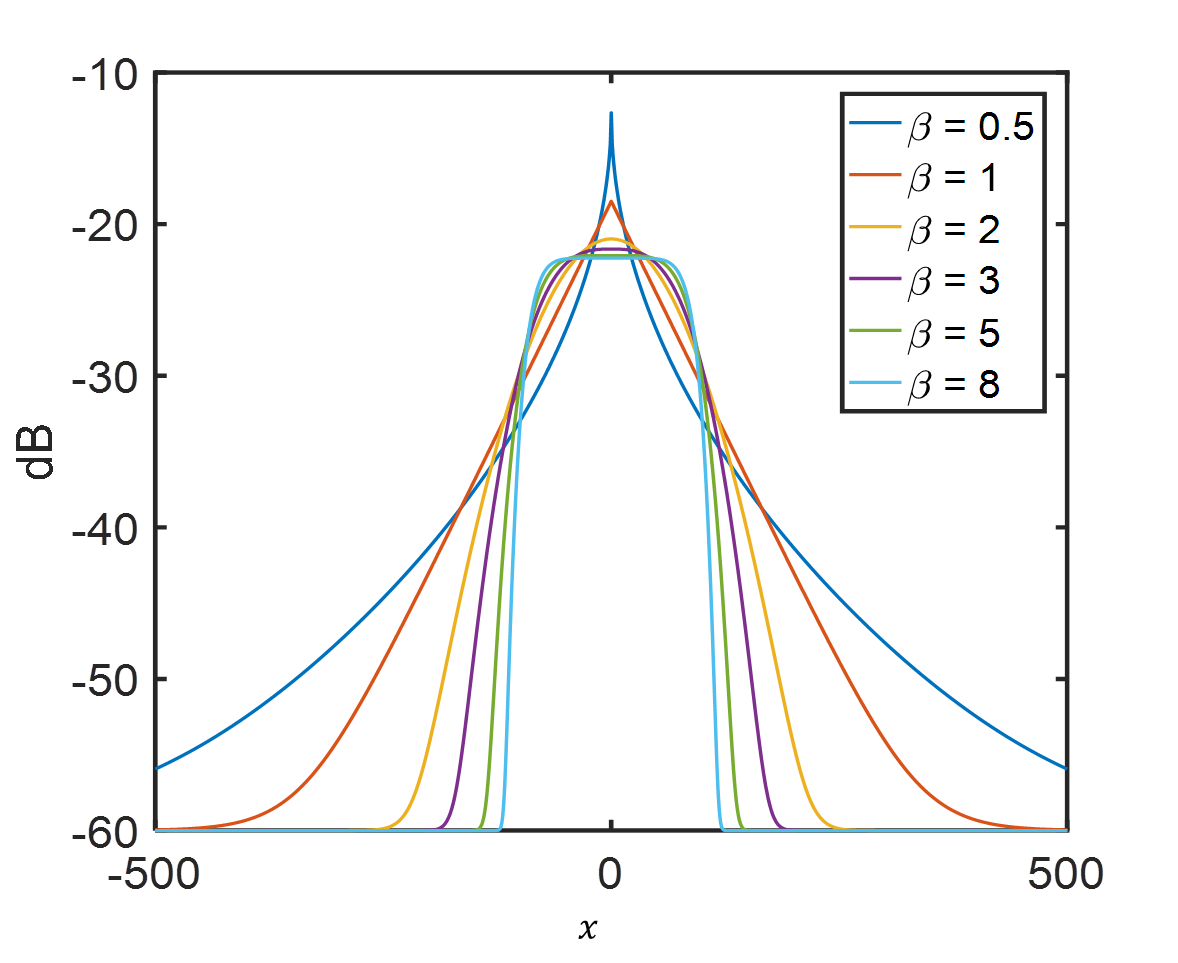
\includegraphics[scale=0.35]{fig_GGD_plot.png}
\par\end{centering}
\caption{Examples of GG functions for varying shape parameter $\beta$.}
\label{fig:GGD_plot}
\end{figure}
%%%%%%%%%%%%%%%%%%%%


\subsection*{Voigt function}

The Voigt function is a convolution of a Gaussian function and a Lorentzian function, which has been widely used for fitting purposes in spectroscopy. The function is given by
%%%%%%%%%%%%%%%%%%%%
\begin{equation}
V(x)= \int_{-\infty}^{\infty} G(x')L(x-x')\,\mathrm{d}x',
\end{equation}
%%%%%%%%%%%%%%%%%%%%,
\noindent where $G(x) = \frac{1}{\sigma\sqrt{2\pi}}e^{-(x-\mu)^2/(2\sigma^2)}$ is the Gaussian PDF and $L(x) = \frac{\gamma}{\pi(x^2+\gamma^2)}$ the centered Lorentzian function. Equivalently, the position parameter $\mu$ can be introduced in the Lorentzian function and the centered Gaussian function can be employed. However, in implementing the convolution, calculation of the Faddeeva function is time-consuming. Therefore, in practical applications, an approximate function, called the pseudo-Voigt function is often used, which is a weighted mixture of the Lorentzian and Gaussian function, with weight $\eta$:%
%%%%%%%%%%%%%%%%%%%%
\begin{equation}
V_{p}(x) = \eta \cdot L(x) + (1-\eta) \cdot G(x),\quad 0\leq\eta\leq1.
\end{equation}
%%%%%%%%%%%%%%%%%%%%


\subsection*{Taylor function}

The Taylor function is the Fourier transform of a specific kind of correlation function. When the correlation function is defined as:%
%%%%%%%%%%%%%%%%%%%%
\begin{equation}
  F_\mathrm{corr}(x) = \exp\left[-k^2u^2\tau^2\left(\frac{x}{\tau}-1+e^{-x/\tau}\right)\right],
\end{equation}
%%%%%%%%%%%%%%%%%%%%
\noindent defining $\Delta = k^2D = k^2u^2\tau$, where $D = u^2\tau$, the above expression becomes:%
%%%%%%%%%%%%%%%%%%%%
\begin{equation}
  F_\mathrm{corr}(x) = \exp\left[-\Delta(x-\tau+e^{-t/\tau})\right].
\end{equation}
%%%%%%%%%%%%%%%%%%%%
\noindent Then the Taylor function is the Fourier transform of $F_\mathrm{corr}$ and acquires the following form:%
%%%%%%%%%%%%%%%%%%%%
\begin{equation}
  T(x) = \mathrm{FFT}\left\{\exp\left[-\Delta_{BB}(t-\tau_{BB}+e^{-t/\tau_{BB}})\right]\times\delta\varphi\right\},
\end{equation}
%%%%%%%%%%%%%%%%%%%%
\noindent where we have introduced the position parameter by adding $\delta\varphi = \exp(i2\pi\mu t)$. The high flexibility of the Taylor function is shown in figure \ref{fig:TD_plot}. Specifically, when $\Delta$ is relatively large ($\Delta = 1$), the distribution shape can vary from Gaussian to Laplacian. At smaller $\Delta$ ($\Delta \simeq 0.1$), the Taylor function resembles the Lorentzian function.

%%%%%%%%%%%%%%%%%%%%
\begin{figure}[h]
\begin{centering}
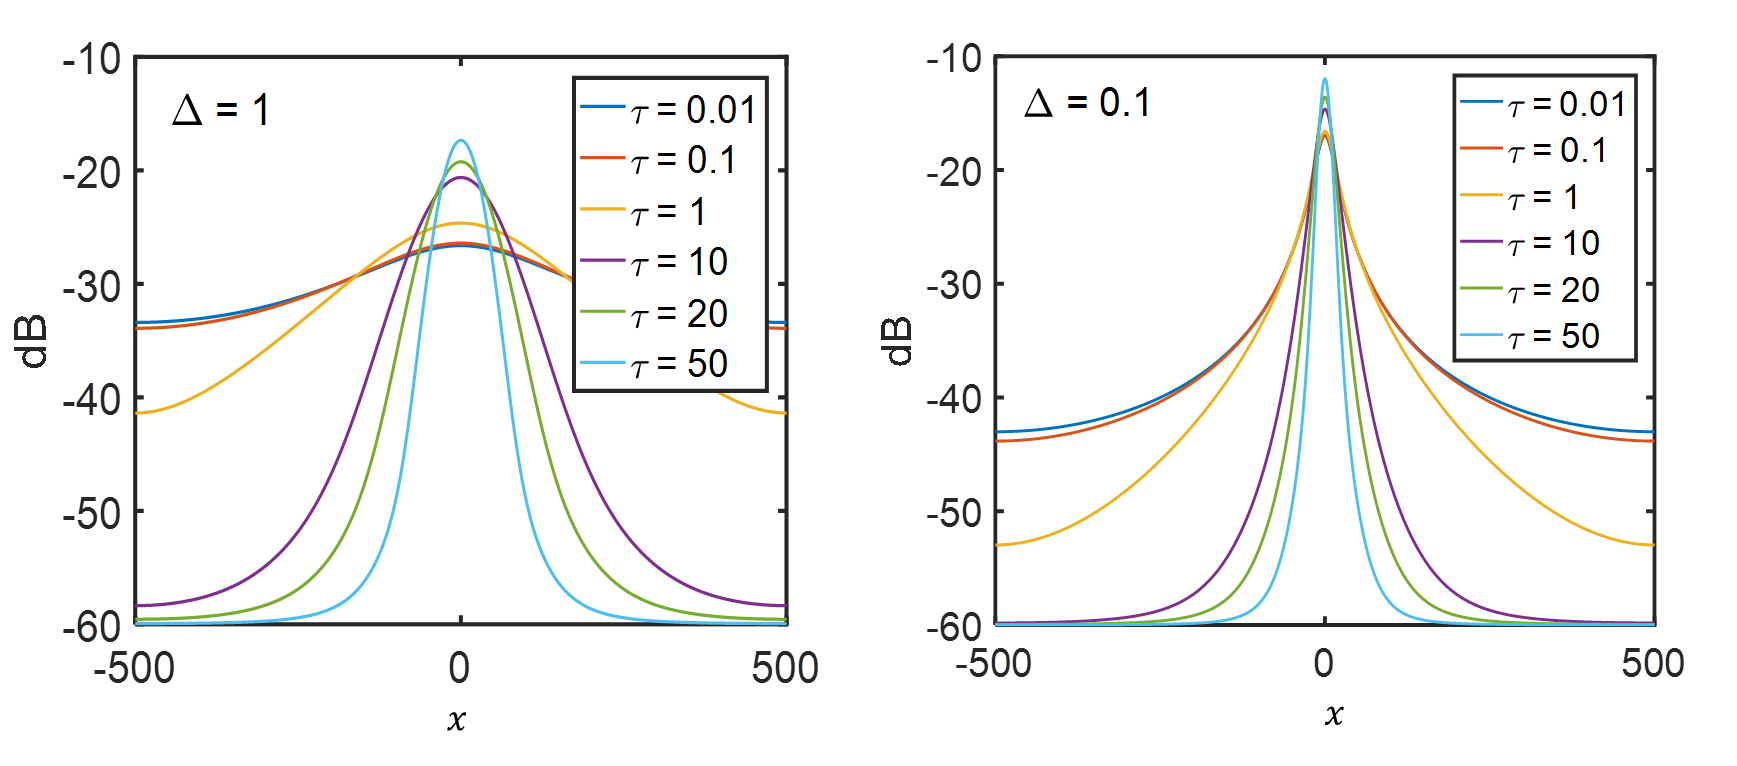
\includegraphics[scale=0.5]{fig_TD_plot.png}
\par\end{centering}
\caption{Examples of Taylor functions with varying $\tau$ at two different values of $\Delta$.}
\label{fig:TD_plot}
\end{figure}
%%%%%%%%%%%%%%%%%%%%



